\section{Resultados}
\FloatBarrier
\subsection{Blur Gaussiano}

La l\'ogica de procesamiento de ambas implementaciones del blur \textbf{no} depende del tipo de im\'agenes, por lo que se procedi\'o a realizar unas pruebas preliminares con distintas imagenes aleatorias y mon\'ocromas. Los tiempos de ejecuci\'on de dichas imagenes resulto ser similar, habiendo peque\~nas diferencias aleatorias que se relacionaron con otras actividades que pudo haber estado realizando el sistema operativo. Por lo que se eligi\'o una de esas im\'agenes al azar para realizar el resto de las pruebas.

Se pudo observar que al realizar el procesamiento con valores de radio chicos (no mayor a 3) los tiempos de ejecuci\'on son similares, esto se asocia al calculo adicion\'al que realiza la implementaci\'on en \textbf{Ensamblador} al momento de procesar las \'ultimas columnas de la sub-matriz se vuelven a procesar reiteradas veces algunos p\'ixeles, pero m\'as que nada se tienen muchos saltos condicionales para no realizar lecturas inv\'alidas. En radios gr\'andes grandes ese procesamiento repetido se vuelve despreciable y se puede apreciar la ganancia de velocidad al realizar muchas menos operaciones de lectura en la implementaci\'on en \textbf{Ensamblador}.
Observamos que, como se hace el c\'alculo de la matriz de convoluci\'on en \textbf{C}, esto tambi\'en puede condicionar un poco los tiempos de ejecuci\'on con imagenes con radio peque\~no, en im\'agnes con radio grande, nuevamente, este valor empieza a tornarse despreciable.

En un principio resulta extra\~no el comportamiento de la implementaci\'on \emph{Ensamblador} con im\'agenes peque\~nas, en la cual los tiempos dieron similares a los de la implementaci\'on \emph{C}, aunque la misma realiza menos lecturas de memoria. Deducimos, entonces, que debido a la cantidad de saltos condicionales que posee dicha implementaci\'on el procesador no puede realizar un manejo de prefetch \'optimo, provocando m\'as estados de espera. Mientras que en la implementaci\'on \emph{C} el compilador realiza optimizaciones y el procesamiento es m\'as secuencial, lo que puede aumentar su performance.

En el resto de los casos el comportamiento es el esperado y solo var\'ia en funci\'on del tamaño de la imagen y del radio. Se conjetura entonces que el rendimiento de los algoritmos est\'a ligado fuertemente a la cantidad de lecturas de memoria, y muy a la cantidad de saltos condicionales en medio del procesamiento.

No se encontr\'o diferencias en los tiempos de procesamiento al cambiar los valores de $\sigma$, esto puede demostrarse por que se utiliza solamente para hacer c\'alculos de la matriz de convoluci\'on, pero no hay saltos ni cambios de l\'ogica que dependan del mismo.

En la figura \ref{fig:figure_blur} se puede observar los resultados de las pruebas realizadas con los diferentes tama\~nos de radio. En los cuales baja el rendimiento con radios peque\~nos (\emph{ASM-S})

%\begin{figure}[htpb]
%    \centering
%    \caption{Tiempo de ejecuci\'on de im\'agenes arbitrarias para el filtro blur con valores arbitrarios }
%    \label{fig:figure_blur}
%    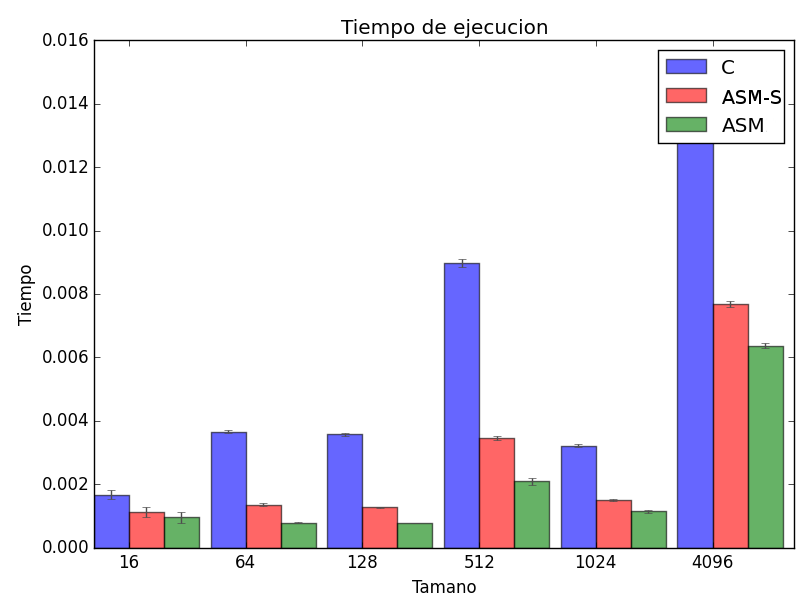
\includegraphics[width=0.75\columnwidth]{include/figure_blur}
%\end{figure}

\FloatBarrier
\subsection{Diferencia de Im\'agenes}

En la primera prueba, para poder notar diferencias significativas. Se ejecut\'o 500 veces cada implementaci\'on del filtro, de esta manera se evita cargar nuevas instancias de los programas y calcular un tiempo incorrecto debido a la carga de d\'isco de las im\'agenes, cache de disco, la invocaci\'on de tareas, y se puede evaluar el uso de cache.

Se utilizaron im\'agenes de diferentes tama\~nos para simular distintos casos y estudiar el comportamiento del filtro. Como el filtro no consiste, ni tiene l\'ogica que dependa del tipo de im\'agen (aleatoria, alto contraste, etc) nos basamos espec\'ificamente en tama\~nos. \\
Cada prueba se ejecut\'o 10 veces, cada una de estas veces se aplic\'o 500 veces el filtro, y se calcul\'o el promedio para el gr\'afico y la desviaci\'on est\'andar que se obtuvo.

En la figura \ref{fig:figure_blur} se puede observar los tiempos y resultados. Se pueden ver los resultados utilizando el \emph{max} inline, que mejora pero muy poco.

%\begin{figure}[htpb]
%    \centering
%    \caption{Tiempo de ejecuci\'on de im\'agenes arbitrarias, para el filtro diff }
%    \label{fig:figure_diff}
%    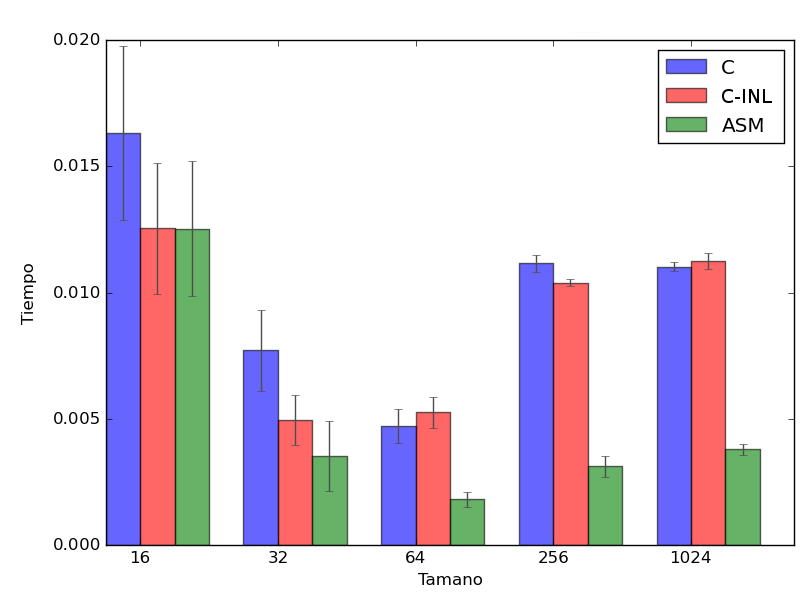
\includegraphics[width=0.75\columnwidth]{include/figure_diff}
%\end{figure}

En la mayor\'ia de los casos los cache-references rondaban el $75.0\%$ mientras que los cache-mises se mantenian menores a $0.05\%$. \\
Puede observarse lo que se hab\'ia predecido en la hip\'otesis, que los tiempos de ejecuci\'on comparados a la implementaci\'on \emph{C} son mucho menores que los tiempos de \emph{Ensamblador}, seguramente debido a la menor cantidad de lecturas de memoria. \\
Tambi\'en se puede conjeturar que influye altamente la cantidad de saltos condicionales y lecturas extras que tiene la implementaci\'on \emph{C} al llamar a la funci\'on \emph{max}.

%TODO CORRER TESTS CON INLINE

Se vi\'o que el tiempo de ejecuci\'on en una imagen de $512x512$ es mucho mayor que $1024x1024$, en especial en la implementaci\'on en C, viendo los datos del cache no pudimos llegar a la conclusi\'on de por que puede funcionar mas lento, ya que los valores son normales y consistentes con las imagenes de $128x128$ y $1024x1024$.

